\documentclass[pageno]{jpaper}

\newcommand{\IWreport}{2018}
\newcommand{\quotes}[1]{``#1''}


\widowpenalty=9999

\usepackage[normalem]{ulem}

\begin{document}

\title{
An Adaptive Strategy for the Competitive Traveling Salesman Problem with Limited Information}

\author{Author: Oluwapelumi Odimayo \\ Adviser: Zachary Kincaid \\ Princeton University Department of Computer Science}

\date{}
\maketitle

\thispagestyle{empty}
\doublespacing

\begin{abstract}
	In this paper, we study an extension of the Traveling Salesman problem titled the Competitive Traveling Salesman in which two agents compete to reach more nodes (objects) in a graph and return to their starting positions finishing the game with, they hope, more payoff than their opponent. Like the traditional Traveling Salesman Problem, this game can be studied through a lens of combinatorial optimization and can be applied to real world applications such as competitive scheduling. \par 
	The rules for this game are straightforward. The players move and make decisions simultaneously, a player may not reverse a move once it has been made, cannot move until they have waited time equal to the distance traveled, and only collects the benefit from a node once they have waited time equal to the previous distance traveled. The total payoff for a player is the total benefit collected minus the total cost accrued during the game. 
	\par We present a novel adaptive strategy for this game that operates in a setting of limited information; players only know which nodes are left unvisited in the graph. This strategy derives a 
	believed state of the opponent and then uses a shallow game tree search to decide whether playing aggressively, beating the opponent to their destination, or playing greedily has a higher expected payoff. A game simulation is implemented to play out pairwise competitions between the adaptive strategy and various greedy strategies. It is shown that the adaptive strategy consistently outperforms a specific set of greedy/low-level strategies.\newline
\end{abstract}
\newpage

\section{Introduction}

The Traveling Salesman Problem (TSP) is a well-known and well-studied NP-Hard problem in combinatorial optimization which has been shown to be applicable to various practical and theoretical situations  \cite{7956764}. It states, given a number of cities and distances between each pair of them, find the shortest tour that visits each city exactly once and returns to the starting position. In this problem, there is a single self-interested agent.\par

The focus of this paper will be a game extension of the traditional TSP termed the Competitive Traveling Salesman Problem (CTSP) which, while theoretical research exists \cite{FEKETE2004377}, \cite{QU20071009}, has not received nearly as much attention as the original problem. This problem arises in various other real-world applications like brand advertising, competitive job scheduling, and (my favorite) elementary school Christmas wrapping paper sell-offs.\par

As a real world source of motivation, consider the analogy of the taxi driver looking to maximize their profit for working in New York City. They get payment for each ride they complete, but must pay for the gas used to travel to their next passenger/assignment. The taxi driver has to consider what passengers they think are worth picking up and if their competition will get to that passenger first. Like the TSP, it is incredibly inefficient for the taxi driver to calculate their optimal tour without competition for large instances, and even harder when other agents are trying to accomplish the same task in a non-cooperative manner. \par

Solutions to the CTSP would be a Nash Equilibrium which would be very difficult to find even in small instances of the game\cite{10.2307/23355415}. It is for this reason that much of the research on this problem seeks to approximate optimal tours using a heuristic approach, much like we've seen in the research surrounding the standard TSP. A very interesting area of this heuristic research is the introduction of adaptive strategies or "hyer-heuristics" that learn/adapt to game situations. By observing the global state of the game, these strategies are able to select what they approximate to be the best possible decision at each step of the game. While this approach has been shown to be successful in academic research, these approaches have traditionally been designed and implemented assuming "complete knowledge". Complete knowledge is the condition that all information about the current state of the game and each agent is known to everyone. In this paper, we want to study how this approach works in a game of incomplete knowledge. Concretely, we want to see how well an agent using an adaptive strategies can perform when they only know their private information and the set of unvisited nodes which is the typical premise in the real world.\par

We focus on a simple 2-Player version of the CTSP game. Each agent tries to visit as many unvisited cities as they can. For each unvisited city $v$ that an agent reaches before their opponent, they will receive some  positive benefit $b(v)$. Furthermore, for each path between cities $(u,v)$ each agent travels along, they pay some cost $c(u,v)$ which is equal to the distance between the two cities.\par

The game ends when there are no more unvisited cities \textbf{and} when both agents have returned to their starting positions. The payoff for each agent \textit{i} is defined as the total benefit they collected minus ther total cost accumulated during their tour. Thus, the ultimate goal for each competing agent is to finish the game with a higher payoff value (total accumulated benefit - total accumulated cost) than their opponent.\par

Direct references are made to approaches used in three research papers that directly study solutions to the Competitive Traveling Salesman Problem. Each paper develops algorithms that construct an adaptive strategy which is then used to compete against greedy/low-level heuristics designed to play the CTSP game to completion. Furthermore, although very similar, each study provides its own version of the CTSP game definition and set of rules followed by the agents, so a brief overview of each of these studies contributions to the work surrounding this problem is given. After this brief overview of past research, a formal definition of the CTSP game used for this study is presented. This is then followed by the approach used to develop our adaptive strategy and the greedy/low-level heuristics used and considered in this setting.\par

In the second half of this paper, we present the formalized algorithm that will construct our adaptive strategy. With this we will also present a formal definition of belief state for the purposes of our algorithm. Then, we will give an overview how we implemented the game simulation along with each of the agent's strategies. We will then go over what metrics were used to evaluate the perfomance of each strategy and then the results of our testing. Finally, we will give a qualitative analysis of some key observations made during experimentation, limitations of our algorithm and setup, and possible avenues for furture work.\newline


\section{Related Work and Motivation}

In 2009, Tomabechi and Fujioka \cite{5228521} presented a novel approach to developing an adaptive strategy for the CTSP. In their paper, they present a simultaneous move search algorithm in which agents play greedily and cancel (reverse) a move if another agent will reach a node before them. They also present a position evaluation method to assist their game simulations in which they hold competitions between computer and human controlled agents. They conclude that their algorithm and position evaluation method can be effectively applied to the CTSP to create consistently well-performing adaptive strategies.\par

Kendall and Li \cite{10.2307/23355415} produced a paper in 2013 in which they describe a hyperheuristic approach to generating adaptive strategies to play  the Competitive Traveling Salesman game against (greedy) opposing agents. This hyperheuristic assumes that the opponent is playing a strategy (or set of strategies) from a limited set of greedy/low-level heuristics. Their initial conclusions were positive and showed that the hyperheuristic was able to perform well under these assumptions. They continued this research in 2017 \cite{7017583} by generalizing their approach to generate adaptive strategies for a variety of games, not just the Competitive Traveling Salesman Problem.\par

While each of these studies produced positive results for the purposes of further studying behavior in the Competitive Traveling Salesman game, they all operate under the assumption of complete information akin to what Uber's alleged "God View"\footnote{https://www.forbes.com/sites/kashmirhill/2014/10/03/god-view-uber-allegedly-stalked-users-for-party-goers-viewing-pleasure/\#7ff4d0131411} would look like if it was fully realized. We look to examine the Competitive Traveling Salesman game under more realistic assumptions on behalf of the agents. It is because of this that we will be conducting this research under the assumption of limited information - agents are only able to see the set of unvisited nodes left in the graph (city). We believe that this will provide a more interesting set of conclusions for the CTSP game and its applications.\newline

\section{Game Definition}

\begin{itemize}
	\item Let $G = (V, E)$ be a \textbf{complete} undirected graph.
	\item $b$ is the benefit function for any vertex $v \in V$
	\item $c$ is the cost function for any edge $e = (u,v) \in E$
	\item $v_{0}$ is the starting position of Player 1.
	\item $w_{0}$ is the starting position of Player 2.
\end{itemize}

Each player plays the game described above using their selected strategy. At the start of the game each player's strategy outputs their first move (the node they will travel to). Each player is restricted to moving only to nodes \textbf{directly adjacent} to their current position in the graph. To travel from $u$ to $v$ in $G$, a player must pay cost $c(u,v)$. Furthermore, a player must wait time $t = c(u,v)$ before collecting the benefit $b(v)$ and selecting the next city they will travel to at which point they're strategy will output their next move. If both players try to collect the benefit from a node at the same time, they will each receive $\frac{b(v)}{2}$. Also note that, for all vertices in the graph, the minimum benefit received from an unvisited city is \textbf{strictly} greater than the maximum cost of traveling to that vertex. Formally, $\forall v \in V$, $b(v) > c(u,v)$. This ensures that each player has incentive to play the game to completion as every move will only increase their payoff.\par

A strategy for this game is defined as some function that takes the current state of the game (or some subset of information derived from the state) and outputs a next move (the node the agent will travel to next). In a game of perfect information, the global state of the game is the same as the information each player knows at each state of the game. This would formally be defined as:\newpage

\textbf{The global state/position of the game:}\newline

\begin{itemize}
	\item $S_{1}$ is the current state of Player 1.
	\item $S_{2}$ is the current state of Player 2.
	\item $U$ is the set of unvisited nodes in the graph $G$.
\end{itemize}

We can see that the global state is simply the current state of each player along with the current set of unvisited nodes in the graph $G$. Strategies in the game of perfect information would take all of this information as input to determine what moves a player would make. In this game of limited information, a player is limited by what they know for sure about themselves and the remaining cities left unvisited. Therefore, their strategies only take in the single player's state and the set of unvisited nodes in the graph $G$ to determine how they will play the game. Formally, the state of the game from a single player's perspective is:\newline

\textbf{Information known to a player $i$:}\newline

\begin{itemize}
	\item $v_{i}$ - Player i's starting position.
	\item $v$ - Player i's current position.
	\item $X$ - The set of consecutive moves made by Player i.
	\item $T_{i}$ - The time Player i must wait before making their next move.
	\item $P_{i}$ - Player i's current payoff.
\end{itemize}

Thus, a strategy for a player $i$ in this game of limited information is some function $F(S_{i}, b, c, U)$ which takes as input player i's state $S_{i} = <v_{i}, v, X, T_{i}, P_{i}>$ and the current set of unvisited nodes in the graph $G$  and outputs a vertex $v^{\prime}$ that will be the next move for the given player. This strategy function effectively takes in a state of a player $S$ and outputs a new state $S^{\prime}$. This definition of a strategy gives us a relationship between consecutive states of the game.\par

We say two states $S$ and $S^{\prime}$ are consecutive if it is possible for the game, subject to the rules previously described, to progress directly from $S$ to $S^{\prime}$. The key constraint here is the parameter $T$ which dictates whether or not a player can make a move to another node in the graph. A player $i$ cannot make a move if $T_{i} > 0$. We separate what state changes are allowed into the following cases:\newline

\textbf{$T_i = 0$ - Player $i$ is allowed to move:}\newline

\begin{itemize}
	\item $v \rightarrow v^{\prime}$ iff $v^{\prime} \in U$
	\item $X^{\prime} = X + v^{\prime}$
	\item $T_{i}^{\prime} = c(v, v^{\prime})$
	\item $P_{i}^{\prime} = P_i + (b(v) - c(u,v))$ where u is the node Player $i$ visited before $v$.\newline
\end{itemize}

\textbf{$T_i \neq 0$ - Player $i$ is not allowed to move:}\newline

\begin{itemize}
	\item $v^{\prime} = v$
	\item $X^{\prime} = X$
	\item $T_{i}^{\prime} = T_i - t$ where $t$ is a single in-game time step.
	\item $P_{i}^{\prime} = P_i$
\end{itemize}

Thus, two Player states $S_i$ and $S_i^{\prime}$ are consecutive iff they satisfy the above constraints. Furthermore, we say two global states $Y = <S_1, S_2, b, c, U>$ and $Y^{\prime}$ are consecutive iff their composing substates are consecutive. Let $Z = $ the number of players allowed to make a move at some poin during the game. We define the state changes of $U$ as follows:\newline

\textbf{$Z = 0$ - No players are allowed to make a move:}\newline

\begin{itemize}
	\item $U^{\prime} = U$\newline
\end{itemize}

\textbf{$Z = 1$ - A single player is allowed to make a move:}\newline

\begin{itemize}
	\item $U^{\prime}= U - $ that player's move
	\item $\forall v \notin U \rightarrow v \notin U^{\prime}$
\end{itemize}

\textbf{$Z = 2$ - All players are allowed to make a move:}\newline

\begin{itemize}
	\item $| U^{\prime} | = | U | - $ those player's moves
	\item $\forall v \notin U \rightarrow v \notin U^{\prime}$
\end{itemize}

Thus, we now have a complete definition of how the global state of the game can change as it progresses. Subject to these rules, we must now construct several greedy/low-level heuristics to play the game "correctly" which will then be used to test our final desired adaptive strategy. In the following section(s) we give the overview of the approach used to develop these strategies.\newline

\section{Approach}

The goal of this research is to translate the complete knowledge adaptive strategies developed in previous studies to this game of limited knowledge. These studies showed that, given complete information, these heuristics could outperform a restricted set of low-level heuristics. The constraint of limited knowledge presents an interesting and novel challenge to CTSP.\par 

We first look to develop a set of greedy heuristics that are relatively reasonable and indeed okay the game to completion. Note that these strategies are not intended to be necessarily good or bad, they are simply strategies that we proposed as generally obvious or naturally employable by someone seeing this game for the first time. The low-level strategies we used to develop our adaptive strategy are:\newpage

\begin{itemize}
	\item \textbf{Highest Benefit} - A pure strategy that takes the state of the game as input and selects the vertex with the highest benefit from the set of unvisited vertices $U$.
	
	\item \textbf{Nearest Unvisited Neighbor} - A pure strategy that takes the state of the game as input and selects the vertext that is the shortest distance away from the the player's current position from the set of unvisited vertices $U$.
	
	\item \textbf{Highest Payoff} - A pure strategy that takes the state of the game as input and selects the vertex that will give the player the highest payoff from the set of unvisited vertices $U$.
	
	\item \textbf{Random} - A mixed strategy which plays one of the previously defined greedy strategies at each decision phase of the game with equal probability.\newline
\end{itemize}

Each of these strategies plays the Competitive Traveling Salesman game essentially with no regard for what the opponising agent might be doing at a given point in time. As a result, these strategies only consider playing the game from a (sub-optimal) single player point of view rather than potentially acting aggressively by attempting to limit the opponent's maximum earning (payoff) potential.\par 

Continuing with this line of reasoning, we seek to design a strategy that still tries to take advantage of the fact that each agent is aware of what nodes are left in the graph. Concretely we want a strategy that:\newline

\begin{enumerate}
	\item Attempts to derive information about the opponent from the available information. (Belief State)
	\item Gains some insight about what strategy the opponent might be playing.
	\item From this information determine whether it is in the agents interest to play aggressively.
	\item Selects the aggressive move if possible, or selects the highest payoff move knowing that the aggressive move is not profitable.
\end{enumerate}

Using these four desirable characteristics as the basis for our adaptive strategy algorithm, we now look to formalize this algorithm. Note that a belief state, because this is a limited information setting and for the purposes of this research, is simply the position an agent believes their opponent is in at any given point during the CTSP game plus the probability that they are playing one of the low-level heuristics.
The final goal is to develop an AI that outperforms this subset of strategies by predicting what strategy their opponent is playing and picking moves that will either, if possible, aggressively cut off the opponent, or select the move with the highest expected payoff under these assumptions.\newline

\section{The Adaptive Strategy Algorithm}

We present an algorithm for our adaptive strategy that is separated into five distinct segments. They are as follows:\newline

\subsection{Initialization}

The initialization step of the algorithm is relatively straightforward. At the start of the game, we assume that the opponent is playing one of the three greedy/low-level heuristics with equal probabibility so we initialize a distribution $D$ of size three with each index containing a value = $\frac{1}{3}$. We initialize the set of nodes for sure visited by the opponent $Q$ to be empty. Next, we initialize a set of "possible moves" $M$ which will hold the moves we believe will be made if the opponent plays each of the greedy strategies. This is initially empty. Finally we initialize some weighting value $W$ which will be used to re-weight this strategy probability $D$ on subsequent iterations of the algorithm.

\subsection{Game Inference}

At each step of the game we want to see if we can derive some information that we know for certain about the opponent. One natural thing to do is to figure out the set of nodes visited by the opponent. We do this by computing the following:\newline

\begin{enumerate}
	\item V = The set of all nodes in the graph. This is implicitly given at the very beginning of the game.
	\item U = The set of all unvisited nodes in the graph.
	\item X = The set of all nodes visited by the agent.
	\item Let Z = V$\backslash$U - The set of all \textbf{visited} nodes in the graph
	\item Let Y = Z$\backslash$X - The set of all visited nodes \textbf{not visited by the agent} $\rightarrow$ The set of nodes visited by th opponent. 
\end{enumerate}

If this set of opponent-visited nodes $Y$ is empty, then play greedily with the \textbf{Highest Payoff} strategy. Otherwise, set the opponent's believed position to be a node drawn uniformly at random from Y$\backslash$Q iff Y$\backslash$Q is also non-empty.

If $M$ is non-empty, record any of the nodes/moves in Y$\backslash$Q that match a move in $M$.

\subsection{Belief State Construction}

If the number of moves matched in $M$ is non-zero re-weight the distribution as follows:

\begin{enumerate}
	
	\item Multiply each probability in $D$ by $W$.
	\item For each correctly guess move in $M$, add $\frac{1 - W}{\# of matched moves}$ to the corresponding index in $D$. (Note that this ensures that the distribution will always sum to 1)\footnote{Other probability weighting functions exist, but this was the simplest to implement and produced positive results for this research. Thank you Professor Kincaid for the tip.}
\end{enumerate}


At this point we will have a probability distribution that gives us a sense for how sure we are that the opponent is playing one of the greedy strategies. We can now go about reasoning through the decision making process for move selection.

\subsection{Shallow Game Tree Search}

This step of the algorithm simply makes two key insights to influence the next move to be output. First, from the opponents (believed) position simulate \textbf{one step} of each of the greedy heuristics. At most there will be 3 different moves output from these simulations. For this implied decision tree:\newpage

\begin{enumerate}
	\item Compute the \textbf{expected payoff} of playing aggressively i.e. trying to cutoff the opponent.
	\item Compute the \textbf{expected payoff} of playing greedily (Highest Payoff) assuming that the opponent's move is no longer possible.\newline
\end{enumerate}

The expected payoff for one possible opponent position is calclated by the formula (for aggressive):

\begin{center}
	$Ex[Agg] = Pr[HB] \cdot Pay(Agg| HB) + Pr[NUN] \cdot Pay(Agg | NUN) + Pr[HB] \cdot Pay(Agg | HP)$
\end{center}

A similar computation can be done for the expected payoff of playing greedily as well.

\subsection{Decision Output}

Select to play the strategy that gives the highest expected payoff (Aggressive vs. Adjusted Greedy). If playing aggressively, select a specific node to travel by selecting a node from $M$ using $D$ as a distribution i.e. \textbf{not uniformly at random}. Otherwise, select the node output by the Highest Payoff heuristic excluding any node we previously determined would be reached by the opponent first.\newline

\section{Implementation}

The entire project was implemented using Python (2.7). The key idea behind the implementation of the game simulation and the players was to make everything as modular as possible, so we implement several different components that, when put together, effectively simulate the Competitive Traveling Salesman game.\par 
In total, the game simulation was implemented with about 600 lines of Python code. We implemented the following elements to construct our CTSP game simulation:

\subsection{random\_player.py}
This is a parameterized player that, depending on input, is able to play any of the pure strategies or the random mixed strategy. The "Player" datatype holds the player's home, position, payoff, time to move, and set of nodes visited. This object implements the function move() which takes as input the set of unvisited nodes in the game and outputs the player's next move auto-updated the player's time until their next move.
\subsection{adaptive\_player.py}
Similar to random\_player.py, this datatype holds the standard information for the player plus the extra objects necessary to perform the adaptive algorithm:

\begin{itemize}
	\item opponent position (int)
	\item strategy distribution (array of size 3)
	\item set of all nodes in the graph (set)
	\item guesses for opponent moves (array of size 3)
\end{itemize}

This object's move() function implements the adaptive algorithm described previously in this report.

\subsection{ctsp.py}

This object/data structure generates the game setup which is essentially a random weighted graph implemented as a two-dimensional array where indeces represent the cost of travel between two nodes. A one-dimensional array is used to store the benfits used for the game as well a set datatype to represent the set of unvisited nodes in the graph.

\subsection{game.py}

This is the game controller which records each player's moves, determines the benefits and cost for each player (subject to the game definition) as well as the total time it takes to complete the game. This implemented as a while loop that terminates when the end-game condition (no unvisited cities left) is met.
\section{Evaluation}

A simple experiment was devised to produce results for this research. We set up games to simulate pairwise competitions for each of the strategies in graphs of size $N = 50$, $N = 100$, and $N = 200$.
We set maximum cost = 100 and maximum benefit = 1,000. Each pairwise competition was run 1000 times and the average payoff for each of these strategies over each of the competitions was recorded. We present the results of these experiments in the following section.

\section{Results}

\figurename{1} shows the results of a pairwise playout of the Competitive Traveling Salesman game. The game was played on graphs of size N = 50, N = 100, and N = 200 respectively; every game was played with the maximum cost equal to 100 and the maximum benefit equal to 1000. The average payoff (against the random player) is reported over 1000 trials of each graph size. This type of experiment was performed against each of the 5 strategies and similar results were found, it is for that reason that we simply included one of these graphs to save space in this report.\par
The most important results/conclusions drawn from these experiments show that our adaptive strategy does indeed perform well against this restricted set of greedy/low-level heuristics. A key observation made from these results is that the adaptive strategy doesn't do any better in larger instances of the game meaning that agent to opponent payoff ratio does not get larger in bigger setting. This is to be expected as our adaptive strategy, while trying to take into account the believed state of the opponent, does nothing to exploit the information given about the remaining nodes left in the graph.\par
Another interesting result that we found was that the adaptive strategy, when playing against itself, did not win or lose by a signifant margin. By this we mean that the results were basically a tie. We do not believe that this means that our adaptive strategy is a best response to itself (we have ideas on how to beat it in the conclusion). Rather, we observed that it makes very poor decisions about where the opponent (the adaptive strategy) would likely move next. 

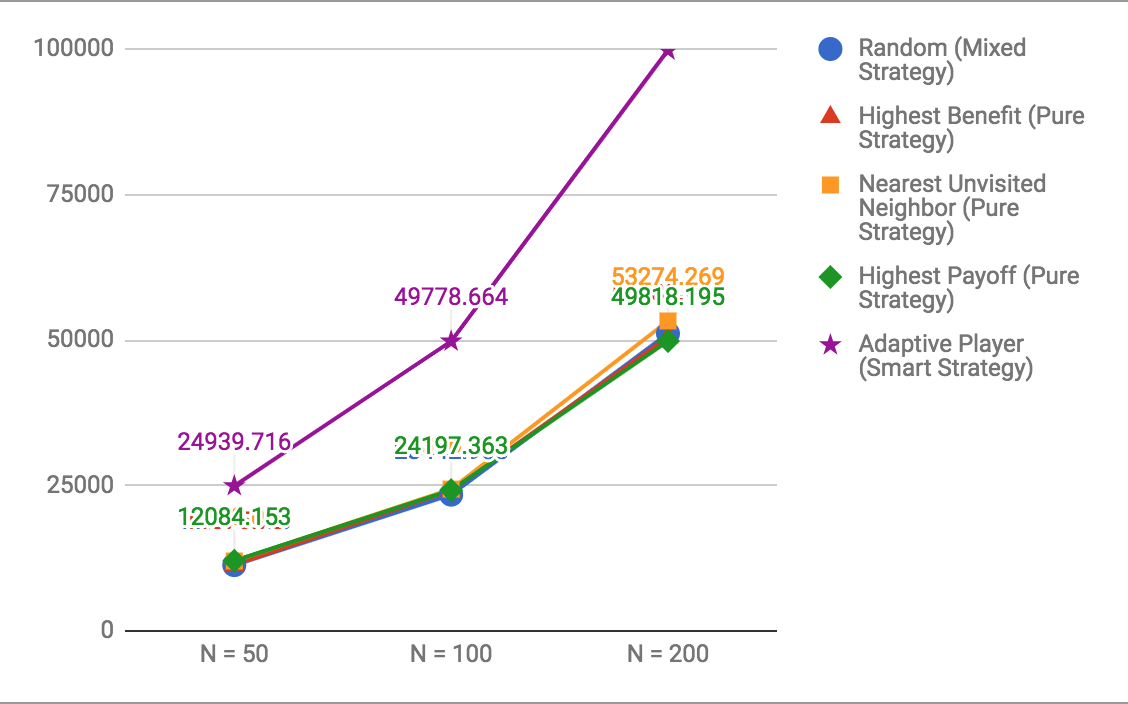
\includegraphics[angle=90, origin=c, width=.90\linewidth]{Results1.png}


\section{Conclusion}

In this paper, we studied the Competitive Traveling Salesman problem, a game extension of the Traditional Traveling Salesman problem in which two agents travel around a city (graph) collect benefit from each node visited, paying a cost to travel between cities, and trying to finish the game with a higher payoff than their opponent. Furthermore, this research focused on a novel setting to the standard CTSP in which each agent only has limited information about the current state of the game.\par
We presented an adaptive strategy that constructs a believed state for the opponent (position and strategy distribution) to inform a shallow game tree search decision problem. The results of this project confirm that this adaptive strategy does indeed perform well in a setting of limited information against a restricted set of greedy/low-level strategies. However, a serious limitation, and an area for possible future work is that this strategy does not do anything to exploit the structure of the remaining cities left in the graph beyond playing aggressively. Another limitation is the re-weighting function used during the belief state construction phase of the algorithm. While clearly effective from the results, it is unclear whether this is an optimal re-distribution function especially in situation involving mixed strategies that use only two of the greedy heuristics.  Furthermore, the greedy strategies are far from optimal, so this might have had an effect on the performance of our adaptive strategy.\par 
Future work will likely involve an implementation of a Monte Carlo Tree Search based hyperheuristic to develop adaptive strategies for the CTSP game in this setting of limited information. Furthermore, the adaptive strategy in this paper could be further expanded upon to derive TSP-based optimal tours for the remaining nodes in the graph or some type of exploitation of this known structure.

A repository containing the code for this project can be found at:\newline
\begin{center}
	\textit{https://github.com/TheColorPlum/IW\_Spring\_2018}\newpage
\end{center} 

\bstctlcite{bstctl:etal, bstctl:nodash, bstctl:simpurl}
\bibliographystyle{IEEEtranS}
\bibliography{references}

\textit{I pledge my honor that I have not violated the University's regulations. - Oluwapelumi Odimayo}
\end{document}

